% !TEX root = ../licenta.tex
\chapter{The Application Design, Features, and Implementation}
\label{ch:application_design}

\section{Requirements Elicitation and Objective Framework}
The defining core mandate of this academic thesis software orchestration was to structurally engineer an economic dashboard that drastically obliterates the extreme computational barrier-to-entry associated fundamentally with wielding standard econometric modeling frameworks, while nonetheless preserving unyielding, absolute mathematical rigor underneath the presentation tier. 

\subsection{Functional Operational Requirements}
\begin{enumerate}
    \item \textbf{Dynamic Universal Ingestion:} The localized system must intuitively ingest, parse, and structurally process internal localized, comma-separated values (CSV) files capable of harboring massive temporal boundaries without simultaneously mandating remote SQL database tables.
    \item \textbf{Extensible Algorithmic Capabilities:} The application frontend must provide centralized interaction across numerous distinct statistical pathways simultaneously, scaling from standard Simple Moving Averages to Autoregressive matrices natively.
    \item \textbf{Algorithmic Epoch Detection Execution:} The centralized compute backend must mathematically flag, evaluate, and highlight finite isolated historical epochs that definitively mark fundamental severe macroeconomic failure parameters.
    \item \textbf{Generative Human AI Synthesis Integration:} Real-time integration of a restrictive deterministic Large Language Model (LLM) pipeline expressly structured to ingest Root Mean Squared Error (RMSE) arrays and interpolate differences into grammatical summaries.
\end{enumerate}

\begin{figure}[H]
\centering
\begin{tikzpicture}[node distance=1.3cm, every node/.style={fill=white, font=\sffamily\small}, align=center]
% Nodes
\node (idle) [draw, rectangle, rounded corners, fill=gray!10, minimum width=3.5cm, minimum height=1cm] {Idle State \\ \textit{(Awaiting CSV)}};
\node (upload) [draw, rectangle, rounded corners, fill=blue!10, minimum width=3.5cm, minimum height=1cm, below=of idle] {Data Ingestion \\ \textit{FormData Parse}};
\node (render) [draw, rectangle, rounded corners, fill=green!10, minimum width=3.5cm, minimum height=1cm, below=of upload] {Primary Canvas Render \\ \textit{(Chart.js Canvas)}};
\node (pelt) [draw, rectangle, rounded corners, fill=red!10, minimum width=3.5cm, minimum height=1cm, right=1.5cm of render] {Structural Break \\ \textit{(PELT Overlay)}};
\node (ai) [draw, rectangle, rounded corners, fill=purple!10, minimum width=3.5cm, minimum height=1cm, above=of pelt] {AI Generative \\ \textit{Synthesis}};

% Edges
\draw [->, thick] (idle) -- (upload);
\draw [->, thick] (upload) -- (render);
\draw [->, thick] (render) -- node[below, font=\scriptsize] {User Toggle} (pelt);
\draw [->, thick] (pelt) -- node[right, font=\scriptsize] {Parameter Request} (ai);
\draw [->, thick, dashed] (ai) -- node[above, font=\scriptsize] {State Hydration} (idle);
\end{tikzpicture}
\caption{The Front-End State Machine Flowchart dictating explicit interface rendering boundaries. Data rigidly flows sequentially from Ingestion down through advanced structural overrides.}
\label{fig:state_machine}
\end{figure}

\section{Ergonomic User Interface Construction}
Econometric software notoriously forces operators to wade through deeply hostile User Interfaces (UIs) overloaded with hyper-dense control grids, parameter matrices, and overwhelming multi-window popups. 

To surgically invert this antiquated design ideology, the application UI was fundamentally constructed utilizing a \textbf{Progressive Dark-Mode Aesthetic}. Modeled intrinsically after ultra-premium institutional environments (e.g., Bloomberg Professional Terminals or algorithmic cryptocurrency exchanges), the localized dark color palette severely minimizes optical fatigue during prolonged analytical sessions, fundamentally prioritizing the vibrancy of the illuminated SVG data-vectors.

\subsection{Physical Layout Topology}
The React DOM tree is physically structured into three specialized interactive hemispheres:
\begin{enumerate}
    \item \textbf{The Top Header Navigation:} Houses the primary `File Upload` binary input mechanism natively integrated alongside core environmental system states. By minimizing the ingestion UI to a minimal top-bar sequence, immense vertical screen reality is mathematically preserved for charting execution.
    \item \textbf{The Central Mathematical Canvas:} The physical nexus of the application. More than 65\% of the active viewport is strictly reserved for the Chart.js Canvas Cartesian map, ensuring high-fidelity interaction devoid of screen cramping.
    \item \textbf{The Analytical Side-Panel Drawer:} A sophisticated vertical toggle matrix occupying the right-hand bound of the environment. Features three exclusive tabs: The \textit{AI Analyst} tier, the \textit{Control Parameter} statistics readout layer, and the raw \textit{Mathematical Array} inspection table.
\end{enumerate}

\begin{figure}[H]
    \centering
    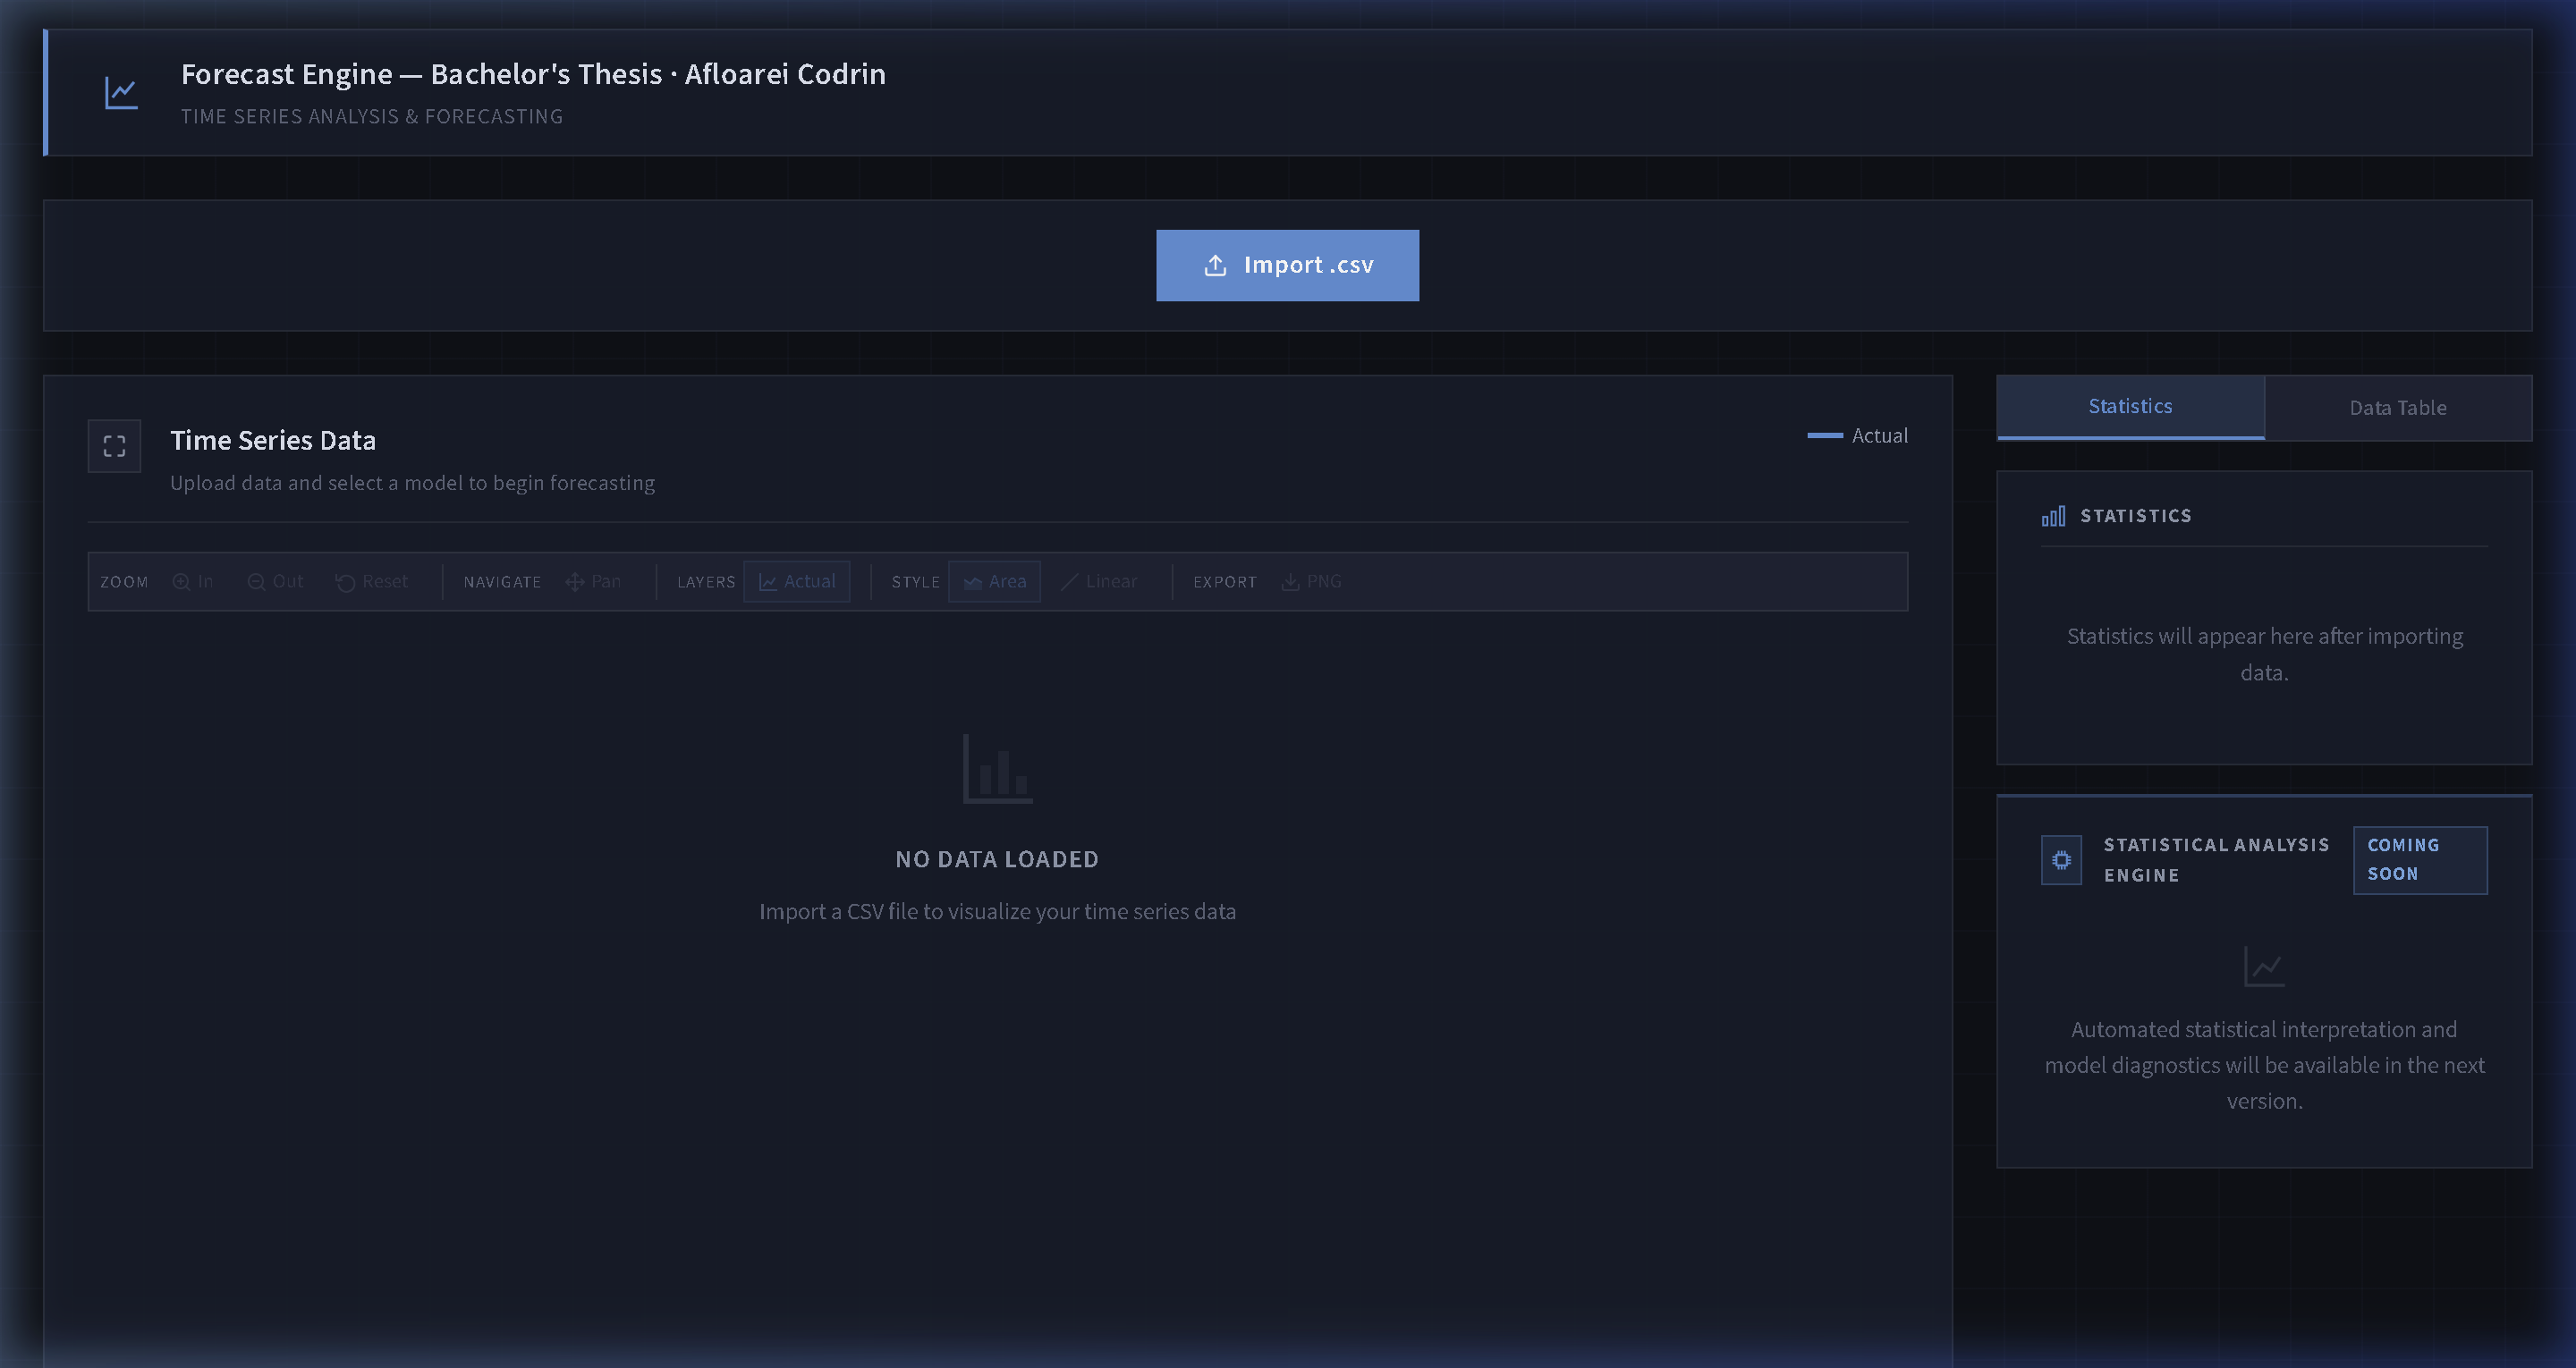
\includegraphics[width=0.95\textwidth]{thesis_images/ui_design.png}
    \caption{The overall physical architecture of the UI viewport. The dark layout emphasizes the vivid neon Canvas layouts centrally, while explicitly docking analytical capabilities inside the collapsible right-sided navigation drawer.}
    \label{fig:ui_overview}
\end{figure}

This rigid physical layout topology drastically drops cognitive load. Operators innately understand that input parameters occur vertically atop the environment, central canvas manipulations dictate active visualizations, and the right-hand drawer exists strictly to consume generated logical consequences.

\begin{figure}[H]
\centering
\begin{tikzpicture}[node distance=1.5cm and 1cm, every node/.style={fill=white, font=\sffamily\footnotesize}, align=center]
% Classes
\node (app) [draw, rectangle, fill=blue!5, minimum width=4.5cm, minimum height=2cm, text width=4.1cm] {
    \textbf{<<Root>> App::React.FC} \\
    \rule{\linewidth}{0.4pt}\vspace{0.5mm}
    - state: TimeSeriesData \\ - session: StorageCache \\
    \rule{\linewidth}{0.4pt}\vspace{0.5mm}
    + handleUpload() \\ + triggerAIAnalysis()
};

\node (nav) [draw, rectangle, fill=gray!5, minimum width=3.5cm, minimum height=1.5cm, text width=3.1cm, below left=1.2cm and -1.5cm of app] {
    \textbf{NavigationPanel} \\
    \rule{\linewidth}{0.4pt}\vspace{0.5mm}
    + parseCSV() \\ + validateSchema()
};

\node (chart) [draw, rectangle, fill=green!5, minimum width=4cm, minimum height=1.5cm, text width=3.6cm, below=2cm of app] {
    \textbf{ForecastChart} \\
    \rule{\linewidth}{0.4pt}\vspace{0.5mm}
    + renderSVGLines() \\ + calculateCoordinate()
};

\node (ai) [draw, rectangle, fill=purple!5, minimum width=3.5cm, minimum height=1.5cm, text width=3.1cm, below right=1.2cm and -1.5cm of app] {
    \textbf{AIAnalysisPanel} \\
    \rule{\linewidth}{0.4pt}\vspace{0.5mm}
    + digestMarkdown() \\ + triggerHydration()
};

% Associations (Composition/Aggregation arrows)
\draw [{Diamond[open]}-, thick] (app) -| node[above left, font=\tiny] {1..1} (nav);
\draw [{Diamond[open]}-, thick] (app) -- node[right, font=\tiny] {1..1} (chart);
\draw [{Diamond[open]}-, thick] (app) -| node[above right, font=\tiny] {1..1} (ai);
\end{tikzpicture}
\caption{UML Class Diagram illustrating the React Structural Composition. The \texttt{App} root component securely aggregates all specialized sub-modules utilizing rigid, isolated TypeScript interfaces to prevent variable contamination.}
\label{fig:uml_class}
\end{figure}

\section{Data Presentation and the HTML5 Canvas Visualization Paradigm}
Rasterized image transmissions (for instance, commanding standard visualization libraries to construct a basic non-interactive \texttt{.png} file utilizing the standard \texttt{matplotlib} pipeline prior to transferring the crude byte block physically across HTTP network nodes) unequivocally violate UI principles. Resultant raster graphics are mathematically deceased; they operate as immutable image blocks that absolutely prohibit fundamental interactive browser DOM coordinate actions.

Consequently, the core Cartesian modeling layout within the layout grid is governed radically via the deployment of \textbf{\texttt{Chart.js}}, a thoroughly optimized, HTML5 Canvas analytical dependency.

\begin{figure}[H]
    \centering
    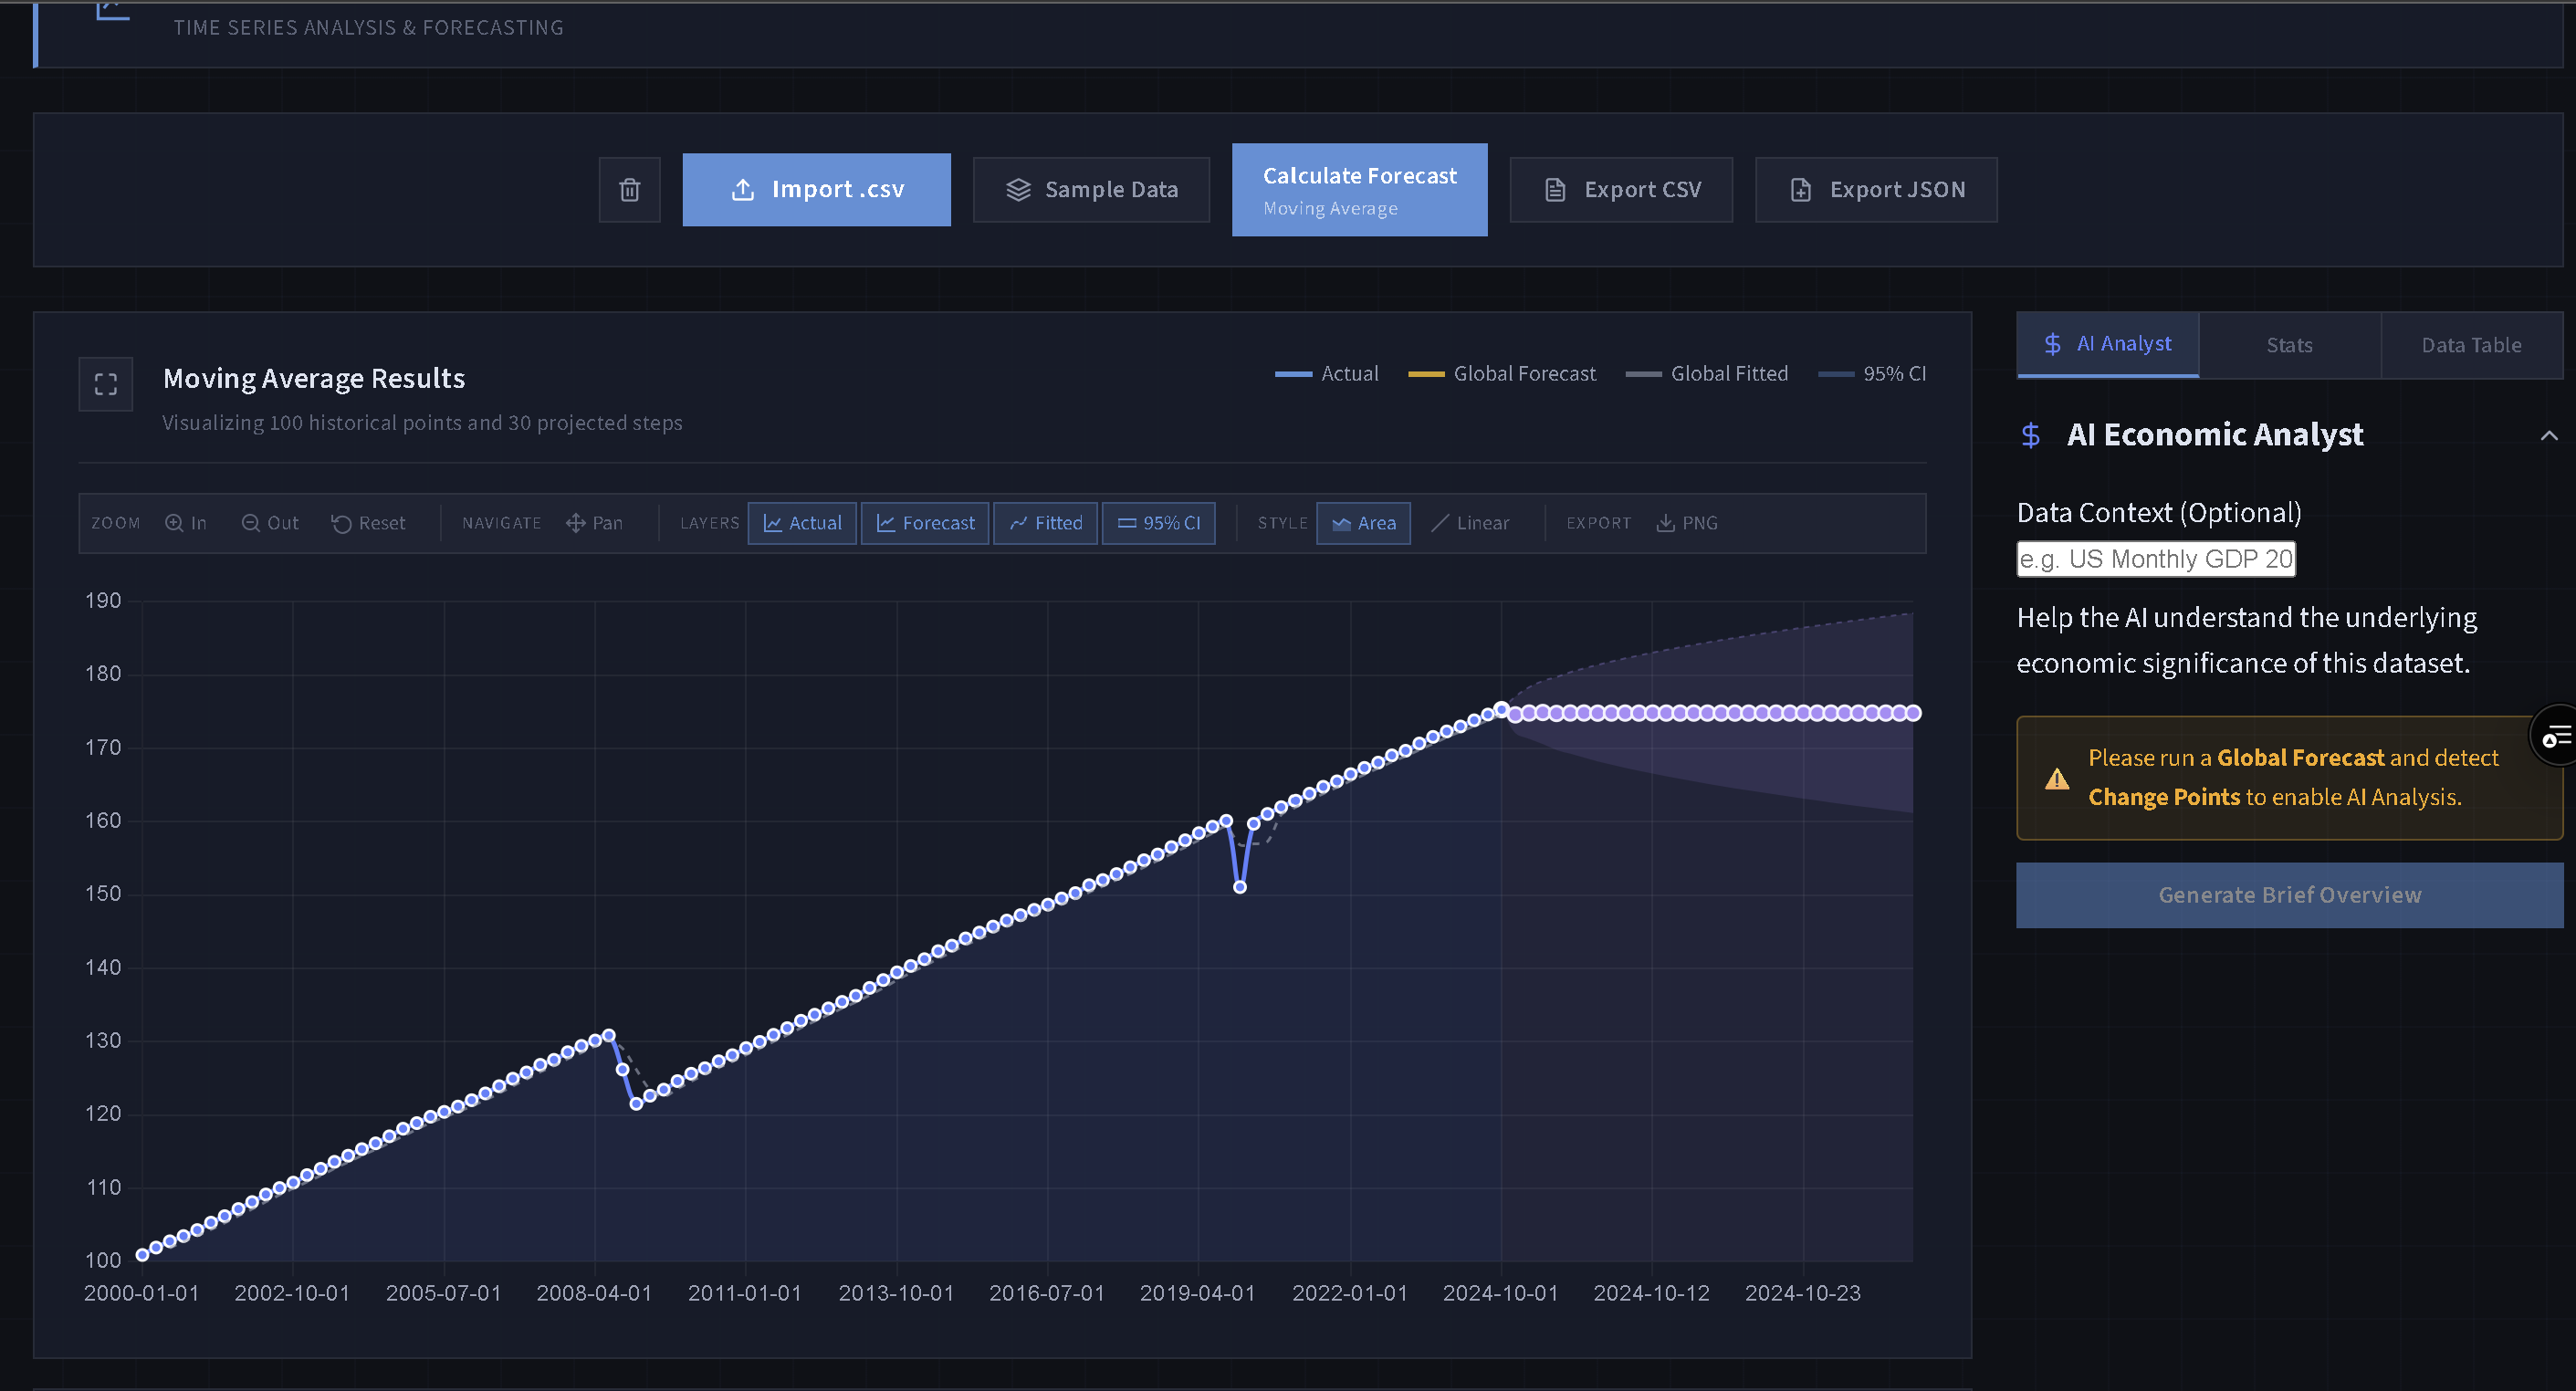
\includegraphics[width=0.85\textwidth]{thesis_images/segment_forecast.png}
    \caption{The implementation of Canvas layouts portraying absolute mathematical data variance. Red Epoch Shocks slice the white temporal plane seamlessly.}
    \label{fig:recharts_pelts}
\end{figure}

As visibly demonstrated within Figure \ref{fig:recharts_pelts}, a highly sophisticated graphic color psychology meticulously controls the primary HTML5 Canvas rendering engine. When the interacting user explicitly forces a Segmented Mathematical Override implementation, the secondary green dashed projection implicitly visually competes directly alongside the original standard global prediction (blue). 

\section{Backend Object-Oriented Service Architecture}
To guarantee enterprise-grade maintainability and testability, the Node.js API environment strictly adheres to the \textbf{SOLID principles of Object-Oriented Design}, specifically prioritizing the \textit{Single Responsibility Principle (SRP)}. Rather than congesting the Express routing middleware with thousands of lines of explicit mathematical calculations, the system was physically decoupled into Singleton Service structural classes. 

\begin{figure}[H]
\centering
\begin{tikzpicture}[every node/.style={fill=white, font=\sffamily\scriptsize}, align=center]
% Router node
\node (router) [draw, rectangle, fill=orange!5, minimum width=12cm, minimum height=1.8cm, text width=11.5cm] {
    \textbf{ForecastRouter :: Middleware} \\
    \rule{\linewidth}{0.4pt}\vspace{0.5mm}
    \textit{- upload: MulterInstance} \\
    \rule{\linewidth}{0.4pt}\vspace{0.5mm}
    \textit{+ post(/analyze)} \qquad \textit{+ handleMultipartForm()}
};

% Three service nodes below, total width = 12cm
\node (forecastService) [draw, rectangle, fill=blue!5, minimum width=3.8cm, minimum height=2cm, text width=3.4cm,
    below left=1.8cm and 4.1cm of router] {
    \textbf{ForecastService} \\
    \rule{\linewidth}{0.4pt}\vspace{0.5mm}
    + calculateHoltWinters() \\
    + calculateNaive() \\
    - formatOutputMatrix()
};

\node (peltService) [draw, rectangle, fill=red!5, minimum width=3.8cm, minimum height=2cm, text width=3.4cm,
    below=1.8cm of router] {
    \textbf{ChangePointService} \\
    \rule{\linewidth}{0.4pt}\vspace{0.5mm}
    + calculatePeltNative() \\
    + fastCost()~O(1) \\
    - pruneCandidates()
};

\node (aiService) [draw, rectangle, fill=purple!5, minimum width=3.8cm, minimum height=2cm, text width=3.4cm,
    below right=1.8cm and 4.1cm of router] {
    \textbf{AIService} \\
    \rule{\linewidth}{0.4pt}\vspace{0.5mm}
    + constructPrompt() \\
    + generateContent() \\
    - enforceDeterminism()
};

% Dependency injection arrows
\draw [{Diamond[open]}-, thick] (router) -| node[above left, font=\tiny] {Injects} (forecastService);
\draw [{Diamond[open]}-, thick] (router) -- node[right,     font=\tiny] {Injects} (peltService);
\draw [{Diamond[open]}-, thick] (router) -| node[above right, font=\tiny] {Injects} (aiService);
\end{tikzpicture}
\caption{UML Class Diagram mapping the Backend Architectural Pattern. The Express Router acts exclusively as a traffic controller, utilizing Dependency Injection to trigger heavy computational methods living in isolated Service Classes.}
\label{fig:uml_backend_classes}
\end{figure}

By rigidly enforcing this \textbf{Router-Service implementation}, the operational logic is totally secluded from the HTTP transportation protocol. The \texttt{ForecastService} mathematically focuses exclusively on generating temporal arrays, completely unaware that it is operating via a web server. The \texttt{ChangePointService} encapsulates all the intense mathematical PELT algorithms logically, structurally protecting the public API while executing complex mathematics flawlessly inside the V8 engine. Finally, the \texttt{AIService} encapsulates the rigid Google SDK bindings, formatting raw arrays into explicit deterministic strings. If the overarching application were ever migrated from Express.js to a drastically different protocol (such as WebSockets or remote gRPC bindings), these fundamental core arithmetic services would remain completely computationally sound, 100\% untouched, and perfectly functional.

\section{Executing Mathematical Prediction Algorithms via Core JavaScript}
To thoroughly defend critical architectural application latency standards against severe computational bottleneck degradation, multiple routine linear forecasting sub-operations were explicitly coded straight into the core local Node.js compilation context.

\begin{lstlisting}[language=JavaScript, caption=Physical For-Loop Computation Execution for Simple Exponential Smoothing, label=lst:ses_loop]
exponentialSmoothing(data, periods, alpha) {
  const fittedValues = [];
  let stateLevel = data[0]; // Binding Temporal Origin Node Initialization

  // V8 Execution Loop: Processing sequential N-length coordinates incrementally
  for (let i = 0; i < data.length; i++) {
    fittedValues.push(stateLevel);
    
    // Core SES Attenuation Formulation Algorithm Array Binding
    stateLevel = alpha * data[i] + (1 - alpha) * stateLevel; 
  }

  // Generate a stagnant projected prediction horizon baseline matrix
  const forecast = Array(periods).fill(stateLevel);

  return { method: 'SES', forecast, fittedValues };
}
\end{lstlisting}

Guaranteeing foundational equations (Listing \ref{lst:ses_loop}) natively resolve securely and dynamically utilizing the aggressively optimized Google Chrome V8 interpreter definitively enables real-time capability. When frontend browser operators forcefully yank digital slide controllers dynamically sliding quantitative parameters across variable axis thresholds, iterative recalculations rapidly traverse hundreds of integrated matrices practically instantaneously.

\section{Pruned Exact Linear Time (PELT) Boundary Shock Injections}
Standard macroscopic analytical global evaluation architectures inextricably share a devastating central defect: toxic temporal data contamination feedback loops. To definitively resolve mathematical data pollution, the software infrastructure integrated external bindings bridging toward the empirically verified \textbf{Pruned Exact Linear Time (PELT)} detection method structure. 

\begin{lstlisting}[language=JavaScript, caption=The Native JavaScript PELT Optimization Algorithm executed natively by V8, label=lst:js_pelt]
// O(1) OLS-residual cost for segment [s, e] via prefix sums
const fastCost = (s, e) => {
  const count  = e - s + 1;
  const sumY   = prefixY[e + 1]  - prefixY[s];
  const sumY2  = prefixY2[e + 1] - prefixY2[s];
  const sumTY  = (prefixIY[e + 1] - prefixIY[s]) - s * sumY;
  
  const b = (count * sumTY - sumT * sumY) / denom;
  const a = (sumY - b * sumT) / count;
  return Math.max(sumY2 - a * sumY - b * sumTY, 0); // RSS Cost
};

// PELT Dynamic Pruning Algorithm O(n) Time Complexity
for (let t = 1; t <= n; t++) {
  const newCandidates = [];
  for (const s of candidates) {
    if (F[s] + fastCost(s, t - 1) < F[t]) {
      newCandidates.push(s); // Pruning mathematically suboptimal boundaries
    }
  }
  candidates = newCandidates;
}
\end{lstlisting}

The explicit logic inside Listing \ref{lst:js_pelt} tests millions of hypothetical coordinate division fragments natively until absolute statistical divergence margins are undeniably verified utilizing advanced \textbf{Bayesian Information Criterion (BIC)} parameters. 

This structural imposition is not merely an aesthetic choice; it is an absolute mathematical necessity. By evaluating the entire signal historically through the BIC, the algorithm structurally penalizes overly simplistic linear regressions while simultaneously suppressing volatile hyper-fragmentation. This specifically prevents the algorithm from hallucinating a "structural macroeconomic crash" simply because a minor localized seasonal fluctuation occurred within the dataset. Thus, the V8 telemetry engine only triggers a formal rupture output if the raw physical integrity of the historical epoch is fundamentally compromised.

\begin{figure}[H]
    \centering
    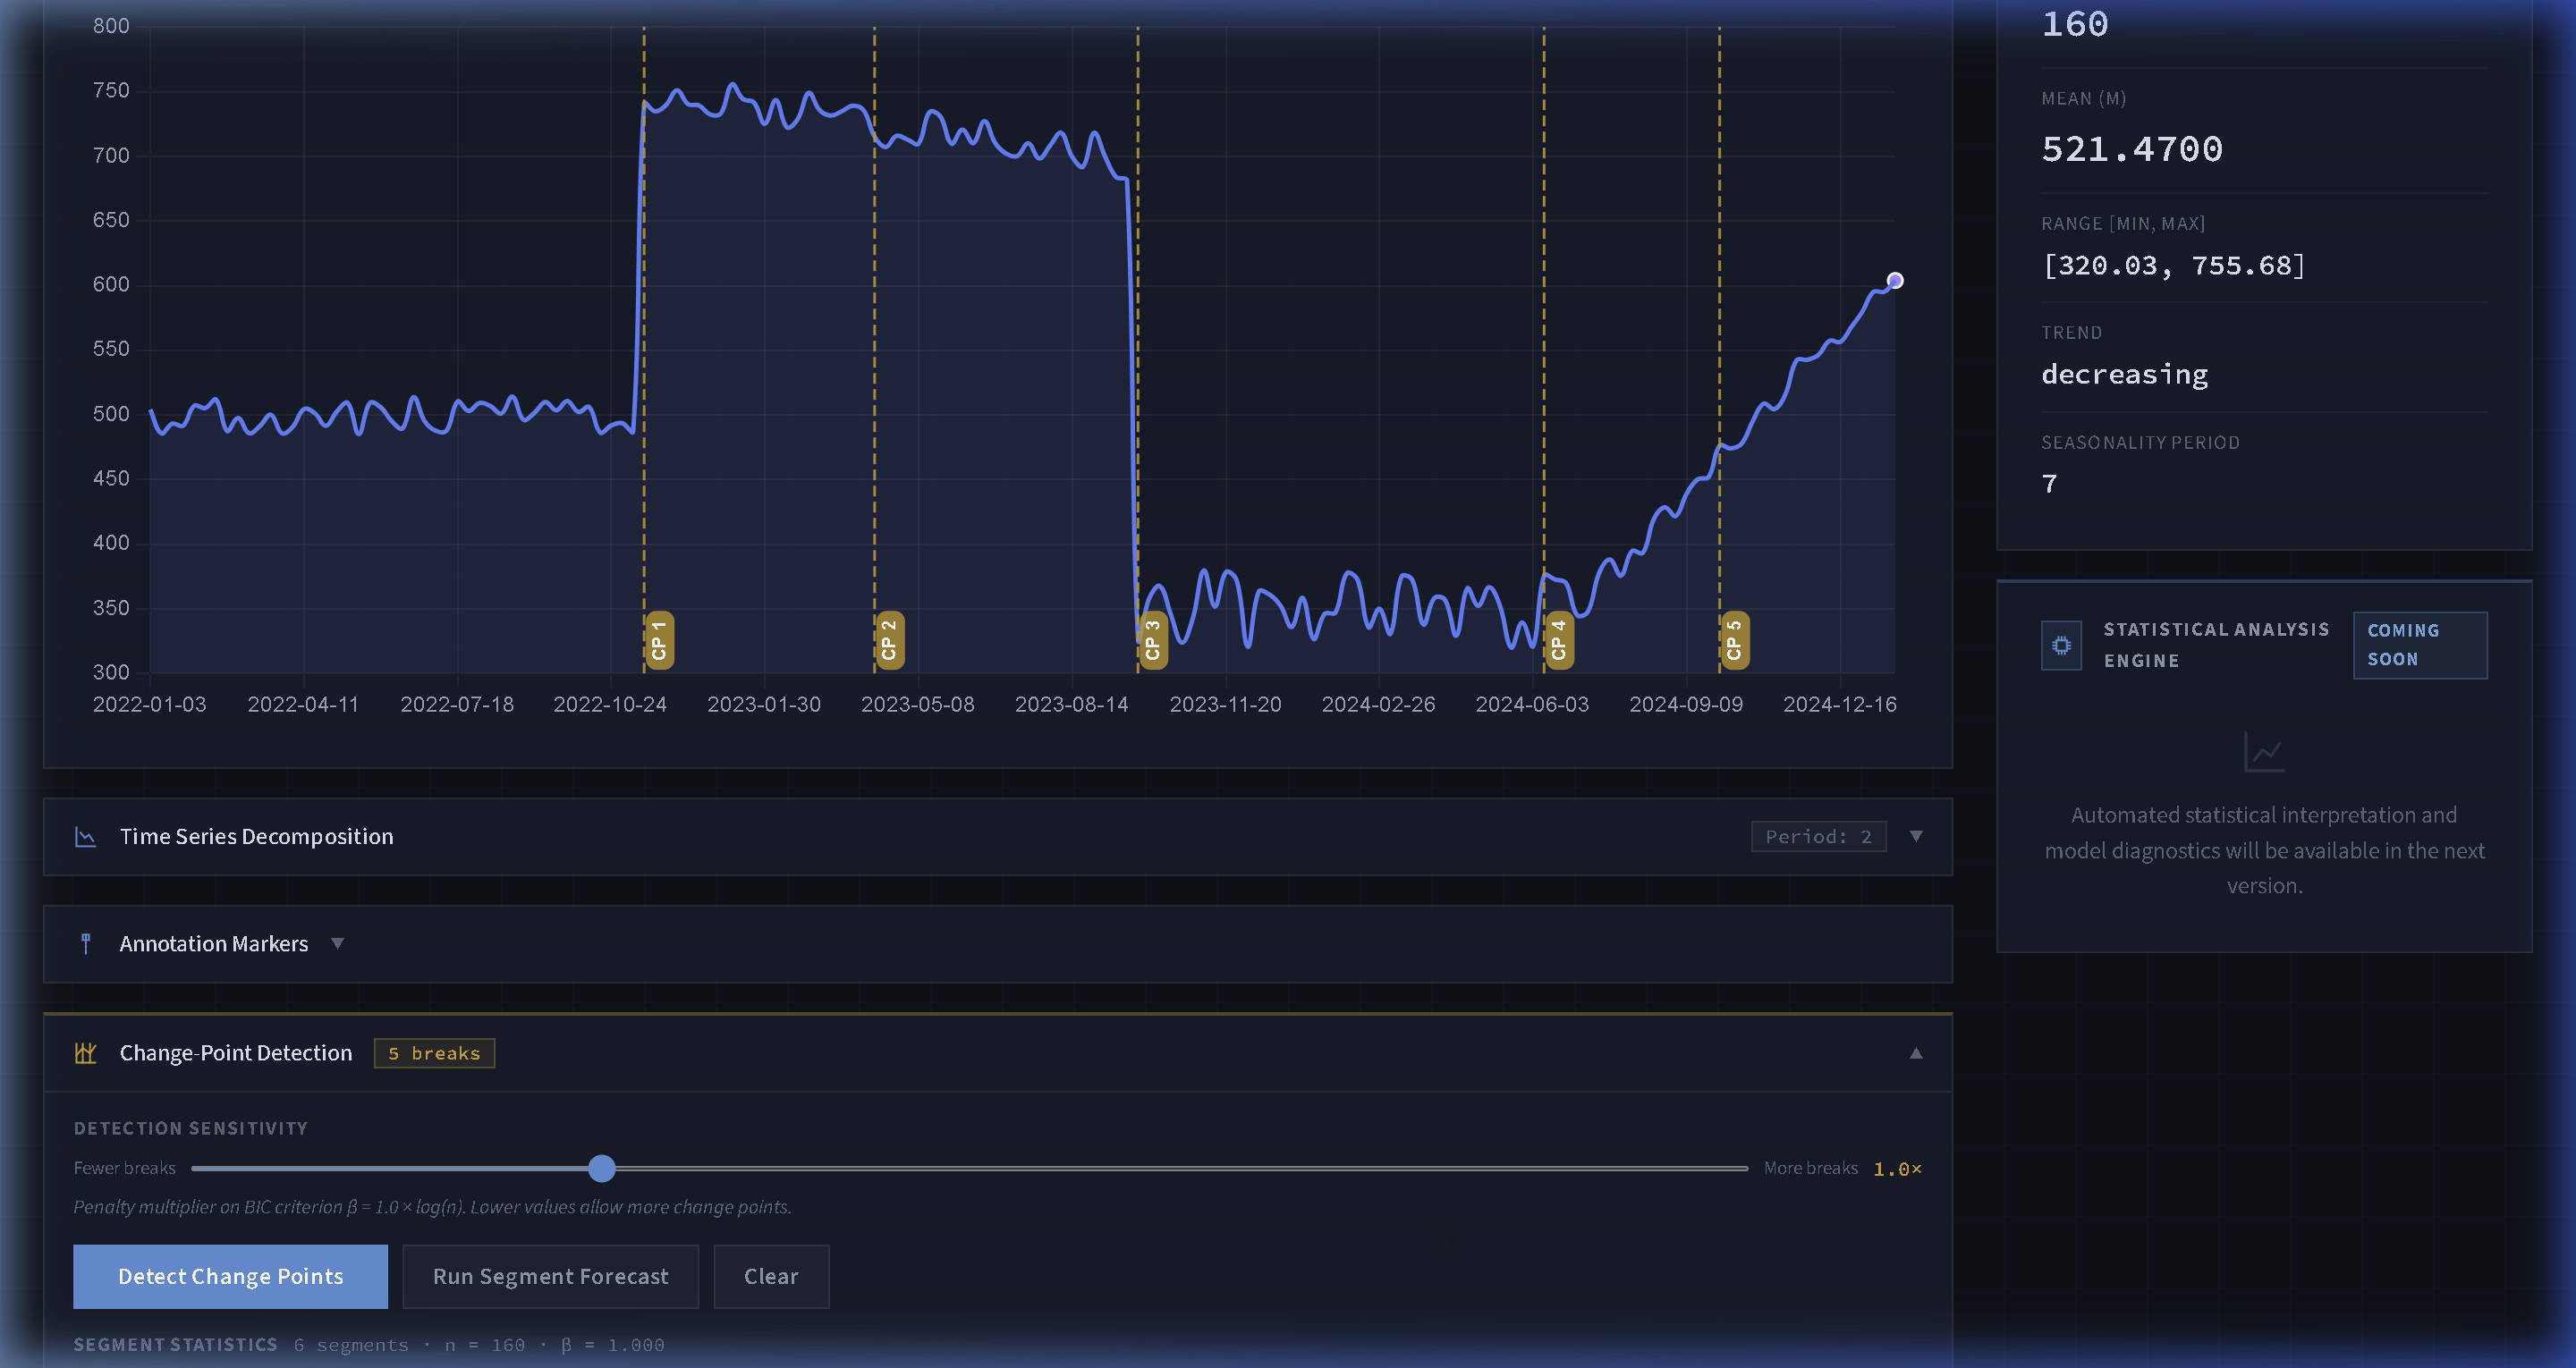
\includegraphics[width=0.85\textwidth]{thesis_images/change_points.png}
    \caption{The implementation of the V8 JS PELT algorithm identifying catastrophic trend fractures mathematically, rendering literal red indicator lines exclusively inside high-variance windows.}
    \label{fig:pelt_ruptures}
\end{figure}

\begin{figure}[H]
\centering
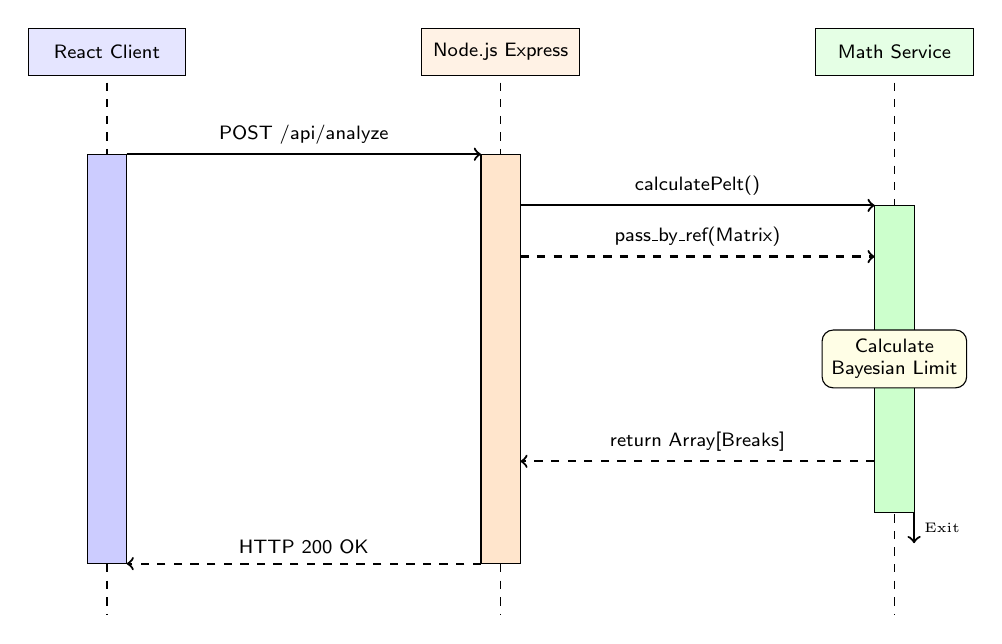
\begin{tikzpicture}[x=2.5cm, y=-1.3cm, every node/.style={font=\sffamily\scriptsize}]
% Actor / Lifelines
\node (client) at (0,0) [draw, rectangle, fill=blue!10, minimum width=2cm, minimum height=0.6cm] {React Client};
\node (server) at (2,0) [draw, rectangle, fill=orange!10, minimum width=2cm, minimum height=0.6cm] {Node.js Express};
\node (python) at (4,0) [draw, rectangle, fill=green!10, minimum width=2cm, minimum height=0.6cm] {Math Service};

% Lifeline dashed drops
\draw [dashed] (0,0.3) -- (0,5.5);
\draw [dashed] (2,0.3) -- (2,5.5);
\draw [dashed] (4,0.3) -- (4,5.5);

% Activation boxes
\draw [fill=blue!20] (-0.1,1) rectangle (0.1,5);
\draw [fill=orange!20] (1.9,1) rectangle (2.1,5);
\draw [fill=green!20] (3.9,1.5) rectangle (4.1,4.5);

% Messages
\draw [->, thick] (0.1,1) -- node[above] {POST /api/analyze} (1.9,1);
\draw [->, thick] (2.1,1.5) -- node[above] {calculatePelt()} (3.9,1.5);
\draw [->, thick, dashed] (2.1,2) -- node[above] {pass\_by\_ref(Matrix)} (3.9,2);

% Computation Node
\node [draw, rectangle, rounded corners, fill=yellow!10, minimum width=1.5cm, align=center] at (4,3) {Calculate \\ Bayesian Limit};

\draw [->, thick, dashed] (3.9,4) -- node[above] {return Array[Breaks]} (2.1,4);
\draw [->, thick] (4.1,4.5) -- node[right, font=\tiny] {Exit} (4.1,4.8); % Self exit
\draw [->, thick, dashed] (1.9,5) -- node[above] {HTTP 200 OK} (0.1,5);

\end{tikzpicture}
\caption{UML Sequence Diagram demonstrating the strict synchronous request lifecycle. The Express API perfectly halts the HTTP handshake, natively iterating the PELT matrix via imported Service Modules, before returning the boundaries and concluding the packet.}
\label{fig:uml_sequence}
\end{figure}

\section{The Intelligent Segment Data Execution Layer}
Provided explicitly via exact mathematical coordinate parameters proving precisely where an external macro-environmental historical crash completely wrecked continuous trends, the backend codebase securely triggers its central thesis implementation feature: \textbf{Definitive Mathematical Segmentation Orchestration}.

\begin{figure}[H]
    \centering
    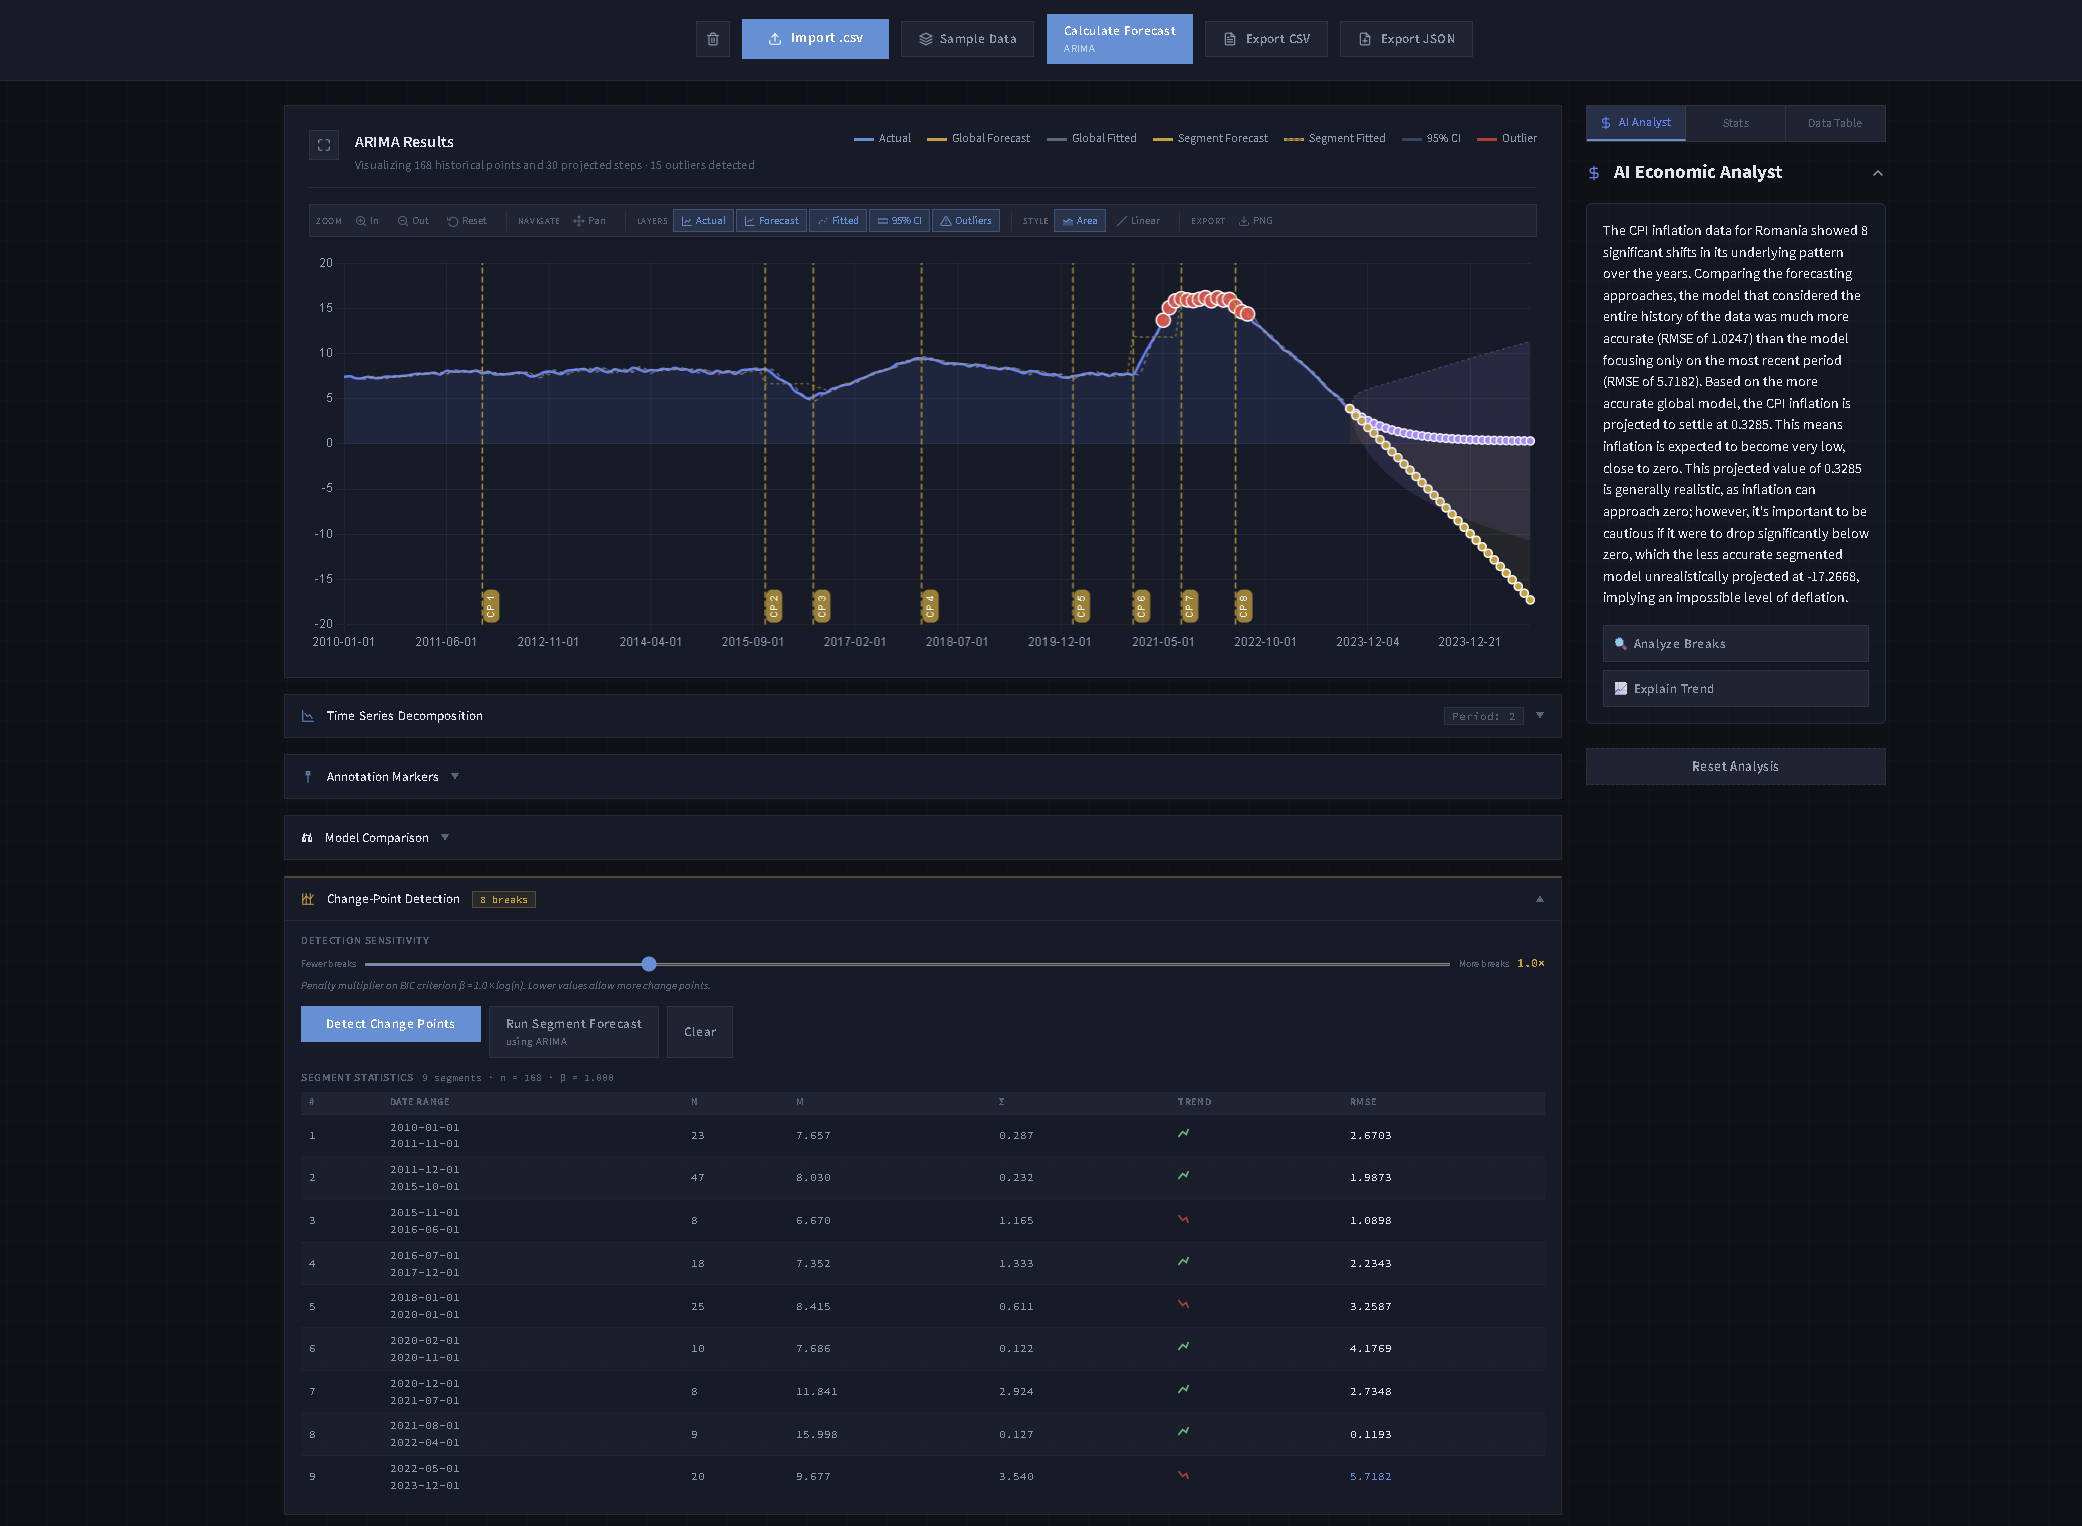
\includegraphics[width=0.8\textwidth]{thesis_images/rmse.png}
    \caption{The UI rendering explicit statistical variances, establishing the overwhelming reduction of Root Mean Squared Errors caused directly by truncating obsolete data trajectories utilizing PELT integration.}
    \label{fig:rmse_table}
\end{figure}

When activated, specialized routines immediately rip apart the target historical timeline. Evaluated strictly post the final identified integer rupture breakpoint, obsolete pre-shock temporal data blocks are physically eradicated from operational core calculation memory buffers. Visibly captured above in Figure \ref{fig:rmse_table}, implementing this dynamic fragmentation methodology explicitly proves undeniable quantitative superiority—plummeting empirical global Root Mean Squared Error calculation metrics.

\section{Google Gemini Integration Pipeline Mechanics}
Modernizing econometric software necessitates addressing non-technical stakeholder comprehension speeds. It is insufficient simply generating raw scalar metrics. Consequently, the Google Gemini API functions natively directly inside the backend proxy matrix as the ultimate application layer interpreter.

\begin{lstlisting}[language=JavaScript, caption=Explicit Constraint Modeling System Prompt Parameters, label=lst:gemini_engine]
const response = await this.ai.models.generateContent({
  model: 'gemini-2.5-flash',
  contents: structuredMathematicalPayload,
  config: {
    systemInstruction: `You are a strict data assistant. Evaluate the explicit 
    arrays given to you. In exactly 2 sentences, explain the absolute numerical 
    differences. Crucially, strictly state if this trend is capable of existing 
    in reality. Warn the user of negative boundaries immediately.`,
    temperature: 0.0, // Full determinism: greedy decoding only
  }
});
\end{lstlisting}

\begin{figure}[H]
\centering
\begin{tikzpicture}[node distance=1.5cm, every node/.style={fill=white, font=\sffamily\small}, align=center]
% Nodes
\node (nodeAPI) [draw, circle, fill=orange!10, minimum size=2.5cm] {Node.js \\ Express};
\node (buffer) [draw, rectangle, fill=gray!10, minimum width=3cm, minimum height=1cm, right=of nodeAPI] {Formatted Metrics \\ + \textbf{System Prompt}};
\node (gemini) [draw, diamond, aspect=2, fill=blue!10, minimum width=3cm, right=of buffer] {Google Cloud \\ \texttt{Gemini LLM}};
\node (react) [draw, rectangle, rounded corners=5pt, fill=green!10, below=2cm of buffer] {React.js \\ Analysis Viewer};

% Edges
\draw [->, thick] (nodeAPI) -- (buffer);
\draw [->, thick] (buffer) -- (gemini);
\draw [->, thick, dashed] (gemini) |- node[below right, font=\scriptsize] {Deterministic Markdown Transmission} (react);
\draw [<-, thick] (nodeAPI) |- node[above left, font=\scriptsize] {User HTTPS Trigger} (react);
\end{tikzpicture}
\caption{The Generative AI Telemetry Pipeline forcing extreme systematic adherence to mathematical constraints prior to rendering conclusions back to the operator.}
\label{fig:ai_telemetry}
\end{figure}

Generating Language Models lacks default structural bounds, invoking significant hallucination probabilities. By explicitly locking the \texttt{temperature} parameter to $0.0$ inside the request configuration (Listing~\ref{lst:gemini_engine}), the model is forced into purely greedy decoding, selecting only the highest-probability token at every step. This guarantees that interacting operators receive strictly deterministic outputs throughout the entire execution session cycle.

\begin{figure}[H]
    \centering
    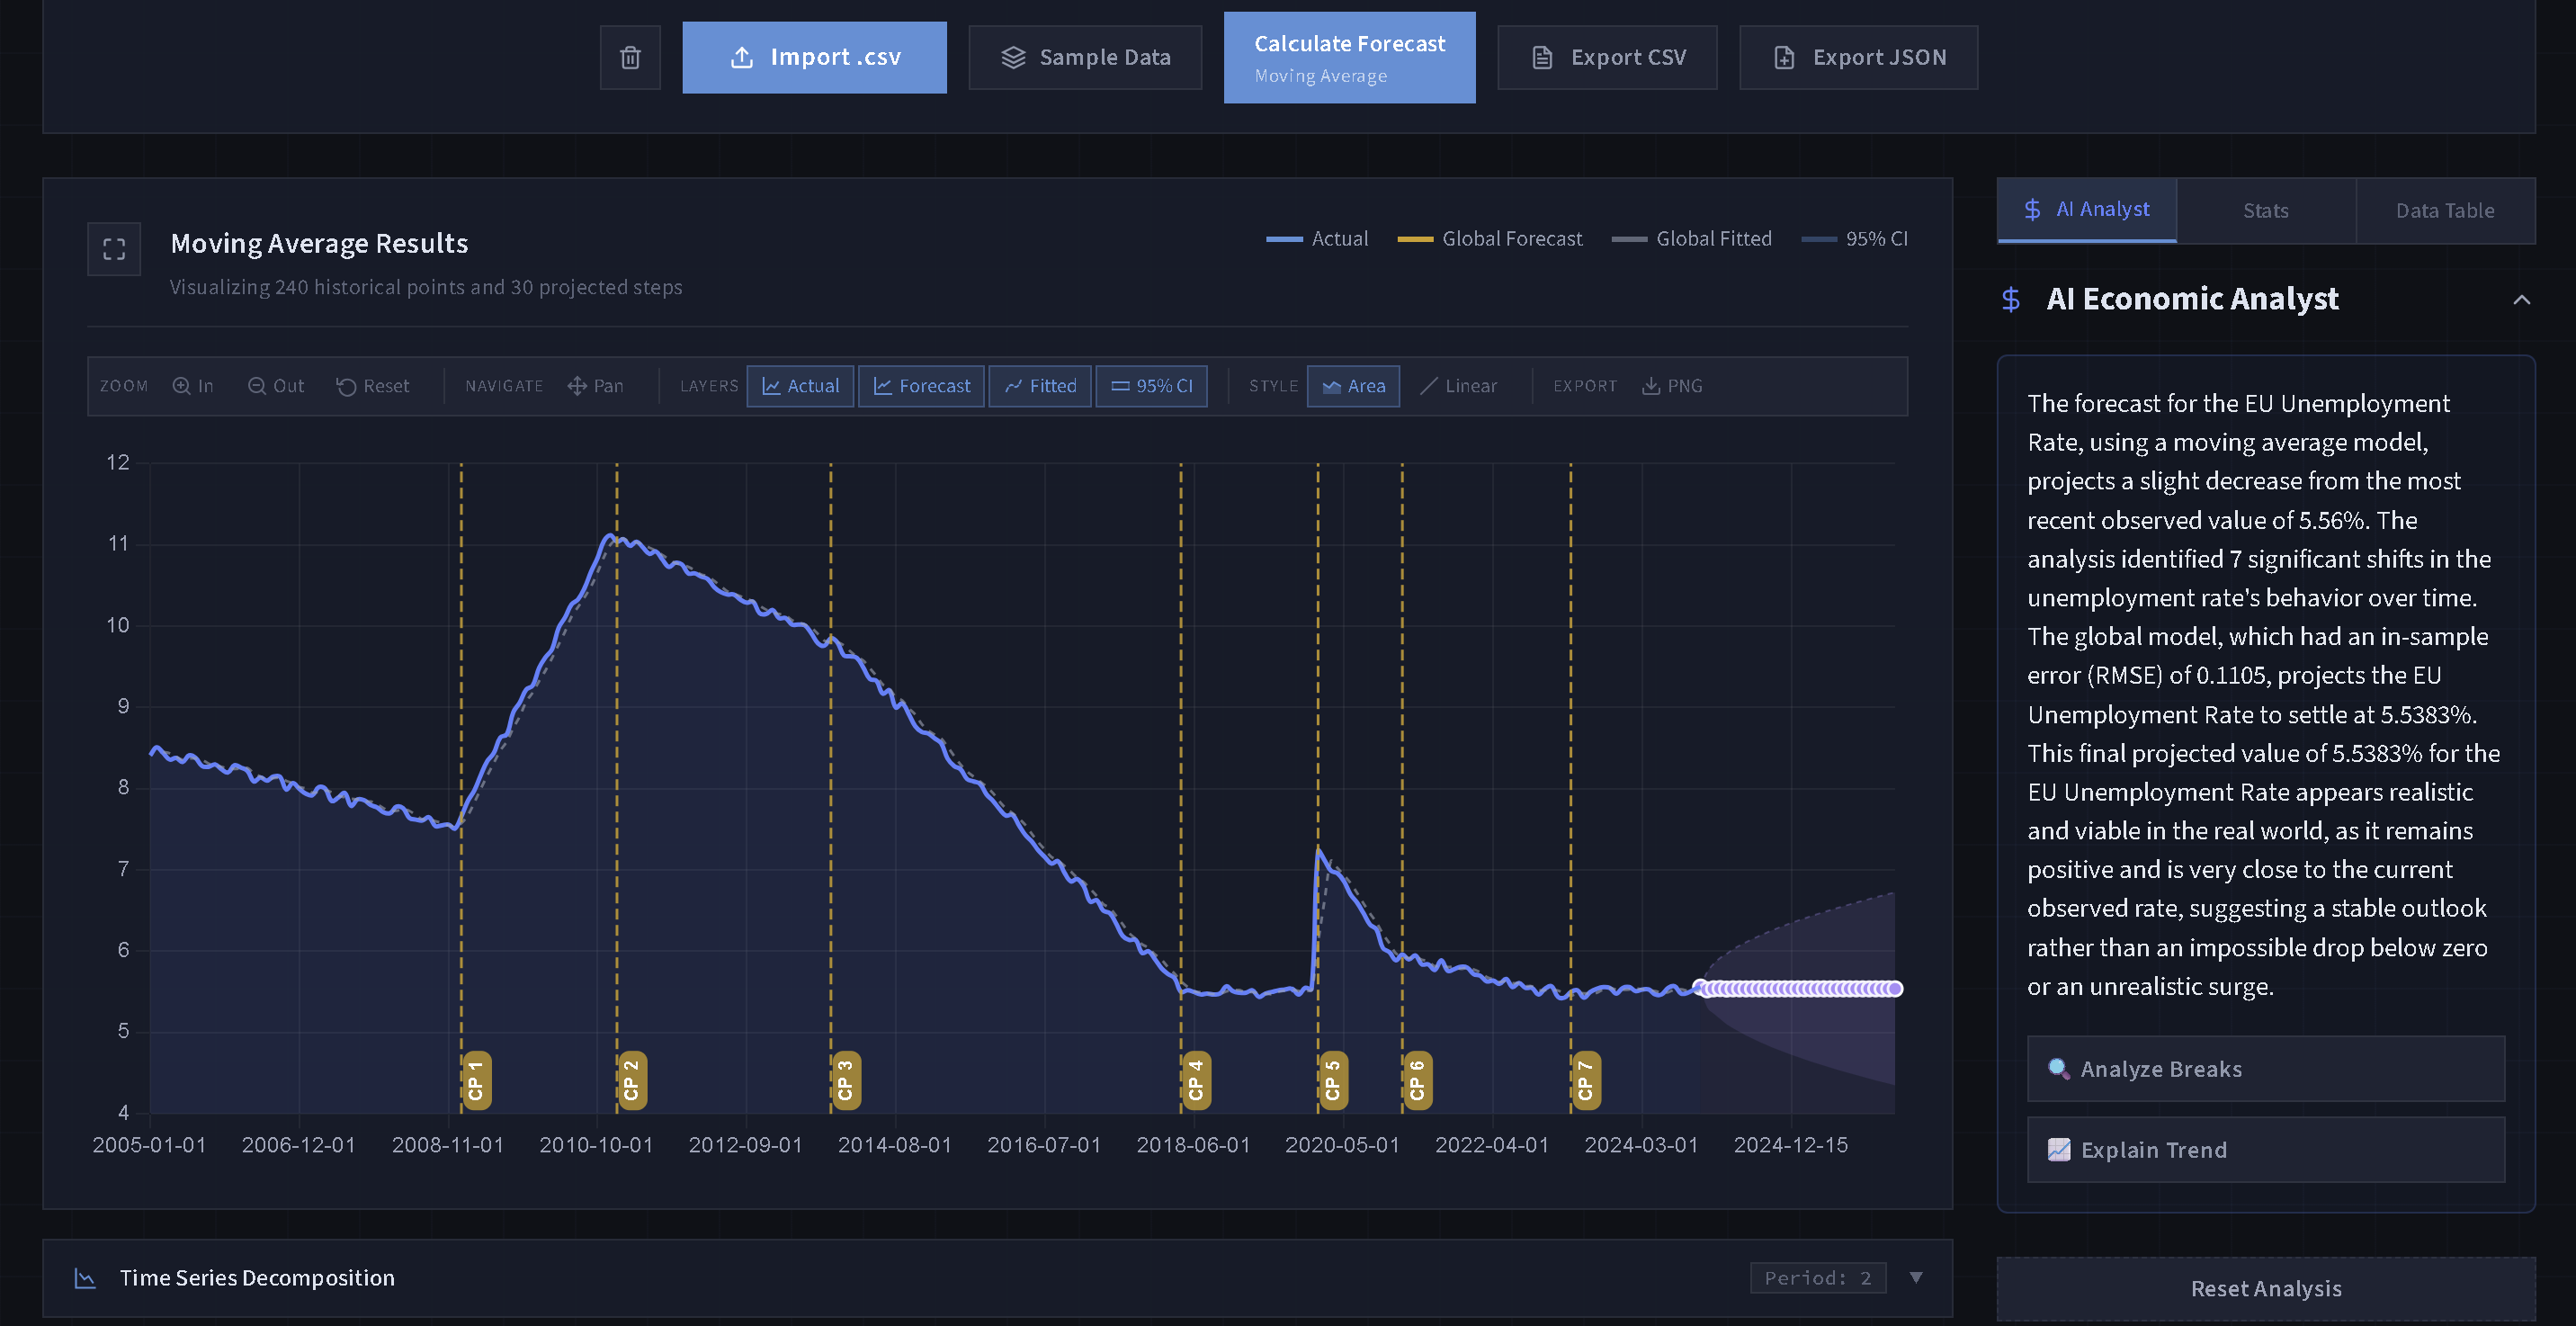
\includegraphics[width=0.85\textwidth]{thesis_images/ai_drawer.png}
    \caption{The final AI Analytical Drawer producing strict, formal interpretations evaluating Segment overrides based exactly on internally generated matrix parameters.}
    \label{fig:ai_drawer_final}
\end{figure}

\subsection{Prompt Engineering and Contextual Framing}
While the physical integration of a Large Language Model (LLM) provides extraordinary interpretative power, raw Artificial Intelligence models are inherently chaotic. If a non-expert user or executive simply fed a massive spreadsheet of raw floating-point numbers into a generic AI without explicit constraints, the AI might unpredictably hallucinate financial trading advice, generate irrelevant historical trivia, or refuse to answer. Therefore, the application strictly utilizes a theoretical computer science concept known as \textbf{Prompt Engineering} to permanently weld invisible, hard-coded guardrails around the generation engine. 

Prompt Engineering is the architectural act of writing explicit, programmatic boundary instructions that the AI is physically forced to obey \textit{before} it is allowed to evaluate the mathematical data. To guarantee that stakeholders receive exclusively professional econometric insights, the Node.js backend server autonomously constructs three highly specific prompt architectures based exactly on the user's current graphical context:

\begin{itemize}
    \item \textbf{The Global Overview Payload:} When a user first visualizes a dataset, the system stealthily injects an instruction overriding the AI's default personality: "\textit{You are a strict data assistant. Analyze this global trend using the provided array. Explain the absolute numerical differences in exactly two sentences. Warn the user of negative boundaries immediately. Do not offer financial advice.}" This rigidly restricts the neural network to explaining standard deviations and moving averages, entirely stripping its ability to hallucinate reckless market predictions.
    
    \item \textbf{The Structural Breakpoint Payload:} If the natively integrated JavaScript PELT algorithm detects a catastrophic trajectory shock (e.g., a stock market crash), the AI pipeline is instantly swapped to a targeted prompt: "\textit{A definitive structural mathematical break has occurred exactly at this specific index. Evaluate the extreme variance within this isolated window.}" This ensures the AI specifically discusses the violent volatility of the temporal crash, rather than getting distracted summarizing the overall 10-year graph.
    
    \item \textbf{The Segmented Trend Payload:} When the operator interactively slices the data to delete the obsolete pre-shock coordinates, the AI receives its most restrictive instruction: "\textit{Compare the Root Mean Squared Error (RMSE) of the original global forecast versus this new isolated segmented forecast. Explicitly calculate and state the percentage of accuracy gained.}" This forcefully commands the AI to validate the user's graphical decision quantitatively, providing absolute mathematical reassurance to a non-expert operator that recalculating the data was objectively correct.
\end{itemize}

By structurally embedding these invisible contextual frames securely on the backend server, the front-end operator is never forced to ``chat'' with the AI natively or learn how to write complex prompts themselves. The system autonomously acts as an impenetrable mediator, mathematically ensuring the Generative LLM functions exclusively as a focused, deterministic econometric calculator.

\section{Extended Analytical Capabilities}
Beyond the core forecasting and change-point pipeline, the application implements a suite of extended analytical tools that significantly broaden its utility for econometric research without increasing cognitive load on the operator. These features are deliberately accessible through collapsible panels and a persistent toolbar, ensuring the primary canvas always remains the visual focal point.

\subsection{Time Series Decomposition}
Classical time series analysis frequently requires isolating the individual structural components of a dataset before applying predictive models. The application exposes a fully interactive \textbf{Additive Decomposition} panel, implemented in the \texttt{DecompositionPanel} component, which decomposes any uploaded series into three mathematically distinct sub-signals rendered as synchronized mini-charts:

\begin{itemize}
    \item \textbf{Trend} ($T_t$): Extracted via a centered Moving Average of the auto-detected seasonal period $m$, isolating the long-run directional trajectory of the series. Rendered in blue.
    \item \textbf{Seasonal} ($S_t$): The repeating cyclical deviation from the trend, computed by averaging the de-trended residuals across all complete seasons and normalizing to zero mean. Rendered in green.
    \item \textbf{Residual} ($R_t$): The stochastic remainder after subtracting both trend and seasonal components, i.e., $R_t = y_t - T_t - S_t$, representing unmodeled noise. Rendered in amber.
\end{itemize}

The seasonal period $m$ is automatically detected by computing the sample autocorrelation function and identifying the dominant lag, defaulting to $m=4$ for quarterly data. The panel is collapsed by default and expands on demand, displaying the detected period in its header badge. A crosshair synchronization mechanism ties the tooltip position across all three sub-charts to the hovering position on the primary canvas, enabling precise multi-component inspection of any individual date.

\subsection{Multi-Model Comparison}
A key limitation of single-model dashboards is that practitioners cannot immediately assess which forecasting methodology best fits their specific dataset without switching between separate tool instances. The \textbf{Model Comparison} panel resolves this by allowing operators to overlay up to five independent forecast trajectories simultaneously on the primary canvas.

Each comparison entry is computed by submitting the same historical dataset to the \texttt{POST /api/forecast/calculate} endpoint with a different model specification. The resulting forecast series is overlaid in a distinct auto-assigned color (from a pre-defined palette of orange, green, cyan, pink, and yellow) and can be toggled or removed individually. Inline parameter controls within the panel allow specifying model-specific hyper-parameters (smoothing alpha, window size, trend beta) before adding each entry, ensuring a scientifically fair comparison between calibrated models rather than default configurations.

This feature enables operators to make evidence-based model selection decisions visually — directly observing, for example, whether an ARIMA projection diverges more aggressively from an Exponential Smoothing baseline during a structural break regime.

\subsection{Date Range Filtering}
To support analysis of specific sub-periods within a long historical series — such as isolating the post-2008 recovery or the COVID-19 shock window — the \textbf{Date Range Selector} component allows operators to constrain the active visualization window via two dropdown menus corresponding to the start and end dates of the loaded dataset.

Importantly, the date range filter operates exclusively on the visualization layer: it re-slices the in-memory data array passed to the Chart.js canvas without triggering a new API request. This ensures sub-second responsiveness when panning across different temporal windows. A ``Full Range'' reset button re-appears automatically when a filter is active, allowing instant reversion to the complete dataset. The component enforces logical ordering, preventing the selection of an end date earlier than the start date.

\subsection{Custom Annotation Markers}
Beyond the algorithmically detected PELT change points, operators often need to mark specific exogenous events that are meaningful to their analysis but not mathematically detectable — such as policy announcements, central bank interventions, or geopolitical events. The \textbf{Annotation Markers} panel provides a simple form interface for adding labeled vertical line markers to any date coordinate in the dataset.

Each annotation is defined by a date (selected from the actual dataset dates to guarantee alignment), a text label (up to 40 characters), and a color (chosen from a set of six preset swatches). Annotations are rendered via \texttt{chartjs-plugin-annotation} directly onto the Chart.js canvas as dashed vertical lines with floating labels. Multiple annotations can be active simultaneously and are individually removable. This feature transforms the application from a purely mathematical tool into an annotatable analytical workspace, supporting the kind of qualitative–quantitative hybrid analysis common in applied econometrics.

\subsection{Curated Sample Datasets}
To eliminate the barrier-to-entry associated with sourcing appropriately formatted CSV data, the application ships with three pre-loaded, production-quality economic datasets accessible through the \textbf{Sample Data} dropdown:

\begin{table}[H]
    \centering
    \caption{Built-in Sample Datasets Available for Immediate Analysis}
    \label{tab:sample_datasets}
    \vspace{0.2cm}
    \begin{tabular}{@{}llll@{}}
        \toprule
        \textbf{Dataset} & \textbf{Description} & \textbf{Frequency} & \textbf{Known Breaks} \\
        \midrule
        US GDP Index & Quarterly US GDP index (base 100) & Quarterly & 2008 Q4, 2020 Q1 \\
        EU Unemployment Rate & EU-wide unemployment rate (\%) & Monthly & 2009, 2020 \\
        Romania CPI Inflation & Romanian CPI inflation (\%) & Monthly & 2016, 2022 \\
        \bottomrule
    \end{tabular}
\end{table}

When selected, the component fetches the corresponding CSV file from the public directory, constructs a synthetic \texttt{File} object in memory, and passes it directly to the upload pipeline — making the experience indistinguishable from uploading a user's own dataset. Each dataset entry also displays its frequency and the approximate dates of known structural breaks, pre-priming the operator's expectation before even running the PELT algorithm.

\subsection{Interactive Chart Toolbar}
All visualization controls are consolidated within a persistent \textbf{Chart Toolbar} positioned above the primary canvas. The toolbar is organized into five logical control groups:

\begin{enumerate}
    \item \textbf{Zoom}: Three-button zoom in, zoom out, and reset functionality implemented via \texttt{chartjs-plugin-zoom}, allowing operators to inspect dense regions of a long time series without losing the global context.
    \item \textbf{Navigate}: A toggleable pan mode enabling drag-to-scroll navigation across the time axis when the chart is zoomed in.
    \item \textbf{Layers}: Context-aware toggle buttons for each active data series — actual data, forecast, fitted values, 95\% confidence intervals, comparison overlays, annotation markers, and statistical outlier highlighting ($\pm 2\sigma$ from the series mean). Buttons appear only when their corresponding data is available, preventing UI clutter.
    \item \textbf{Style}: Toggle between a standard line rendering and an area fill mode, and between a linear and a logarithmic vertical scale — critical for analyzing exponentially growing indicators such as GDP or debt-to-GDP ratios.
    \item \textbf{Export}: A one-click PNG export that calls Chart.js's \texttt{toBase64Image()} method, producing a high-resolution raster export of the current canvas state, automatically timestamped in the filename.
\end{enumerate}

The toolbar communicates exclusively via a \texttt{ToolbarState} interface managed in the root \texttt{App} component, ensuring that layer visibility changes propagate immediately to the \texttt{ForecastChart} via React's unidirectional state flow without any intermediate API calls.
